\documentclass{article}
\usepackage[english,russian]{babel}
\usepackage[utf8]{inputenc}
\usepackage{indentfirst}
\usepackage{graphicx}
\usepackage{float}
\usepackage[margin=2cm]{geometry}

\begin{document}
    \begin{titlepage}
        \begin{center}
            ГУАП
            \vspace{0.25cm}

            КАФЕДРА №51
        \end{center}

        \begin{flushleft}

            ОТЧЕТ

            ЗАЩИЩЕН С ОЦЕНКОЙ

            ПРЕПОДАВАТЕЛЬ


            \vspace{0.5cm}

            $\rule{5cm}{0.15mm}$ \hfill $\rule{2.2cm}{0.15mm}$  \hfill $\rule{3.25cm}{0.15mm}$

            должность, уч. степень, звание \hfill подпись, дата \hfill инициалы, фамилия
        \end{flushleft}


        \hspace{2cm}

        \begin{center}
            ОТЧЕТ ПО ЛАБОРАТОРНОЙ РАБОТЕ №15


            \vspace{1cm}

            HttpSession. CSS


            \vspace{1cm}

            по курсу: ОСНОВЫ ПРОГРАММИРОВАНИЯ {\MakeUppercase{\romannumeral 2}}
        \end{center}

        \vspace{3cm}

        \begin{flushleft}
            РАБОТУ ВЫПОЛНИЛ

            СТУДЕНТ ГР. № 5511 \hfill $\rule{2.2cm}{0.15mm}$  \hfill $\rule{3.25cm}{0.15mm}$

            \hspace{7.8cm} подпись, дата \hfill инициалы, фамилия
        \end{flushleft}

        \vspace{5cm}
        \begin{center}
            Санкт-Петербург 2017
        \end{center}
    \end{titlepage}

    \section{Задание}
    Реализовать сервлет для организации доски объявлений. Объявление содержит текст и заголовок (время размещения и имя пользователя).

    Для того, чтобы разместить, необходимо ввести логин и пароль (пройти аутентификацию). При старте сервлет загружает базу пользователей и их паролей из текстового файла. Просматривать объявления можно без аутентификации (ввода логина и пароля).

    На главной странице находится ссылка “войти в систему” и показывается список объявлений. После входа в систему добавляются ссылки: “выйти из системы”, “добавить объявление”.
    Для аутентификации необходимо использовать класс HttpSession
    Для перенаправления пользователя на другую страницу и включения в  страницу готов кусков html кода можно воспользоваться классом RequestDispatcher
    Протестировать, что при очистке cookie в браузере, пользователь выходит из системы.

    Между перезагрузками сервера (рестарт Tomcat) список объявлений можно не сохранять.

    Дополнительные требования (CSS):


    \begin{enumerate}
        \item Оформление страницы должны быть задано в отдельном файле style.css
        \item Должны быть созданы три стиля:

        \begin{enumerate}
            \item Заголовк объявления
            \item Текст объявления
            \item Ссылка с командой  (“войти в систему”, “выйти из системы”, “добавить объявления”)
        \end{enumerate}
        \item В работе должно быть два варианта оформления (переключение --- переименованием файлов на сервере)
    \end{enumerate}

    \section{Дополнительное задание}
    Создать суперпользователя, который может добавлять и удалять пользователей. 

    \section{Реализация}
    Программа реализована с использованием контейнера сервлетов Apache Tomcat.
    Все классы программы делятся на model, service и web. Model -- представляют собой классы, которые хранят и предоставляют информацию. Service -- классы для имлементации логики классов из Model. Web -- сервлеты, которые принимают и отвечают на запросы клиентов, связаны с .jsp файлами классом RequestDispatcher. 
    Аутентификация в программе происходит в классе LoginServlet с помощью класса HttpSession и его возможности задать параметры сессии. 
Следовательно, сервлеты проверяют параметры сессии для того, чтобы определить тип пользователя.  
	Так, например, выдаются разные Html файлы клиентам, у guest есть только возможность войти в систему, у user есть возможность написать сообщение и выйти из системы, а у admin есть возможности user'a плюс возможность управления аккаунтами пользователей.
	Информация о пользователях загружается из файла data/users в UserService. 
    \section{Инструкция}
    После запуска сервера при посещении страницы localhost:8080/board перед пользователем откроется страница просмотра объявлений. У него есть возможность войти в систему нажав LOGIN в верхней правой части экрана, далее он будет перенаправлен на форму ввода логина и пароля.\\ 	 После успешного ввода данных пользователь переправляется обратно на страницу с объявлениями, только теперь он может добавить новое сообщение, нажав на кнопку ADD MESSAGE. Если пользователь заходит по аккаунтом суперпользователя, то у него появляется кнопка USER MANAGEMENT, которая отправляет пользователя на страницу со списком всех пользователей, он может удалить одного из них, нажав на соответствующее имя или же может добавить пользователя, нажав на кнопку ADD NEW USER.
    \section{Тестирование}

    \subsection{Главная страница}
    При запуске приложения нам предлагается страница без объявлений.
    Мы можем просматривать объявления как гость или залогиниться. 
    \begin{figure}[H]
        \begin{flushleft}
            \centerline{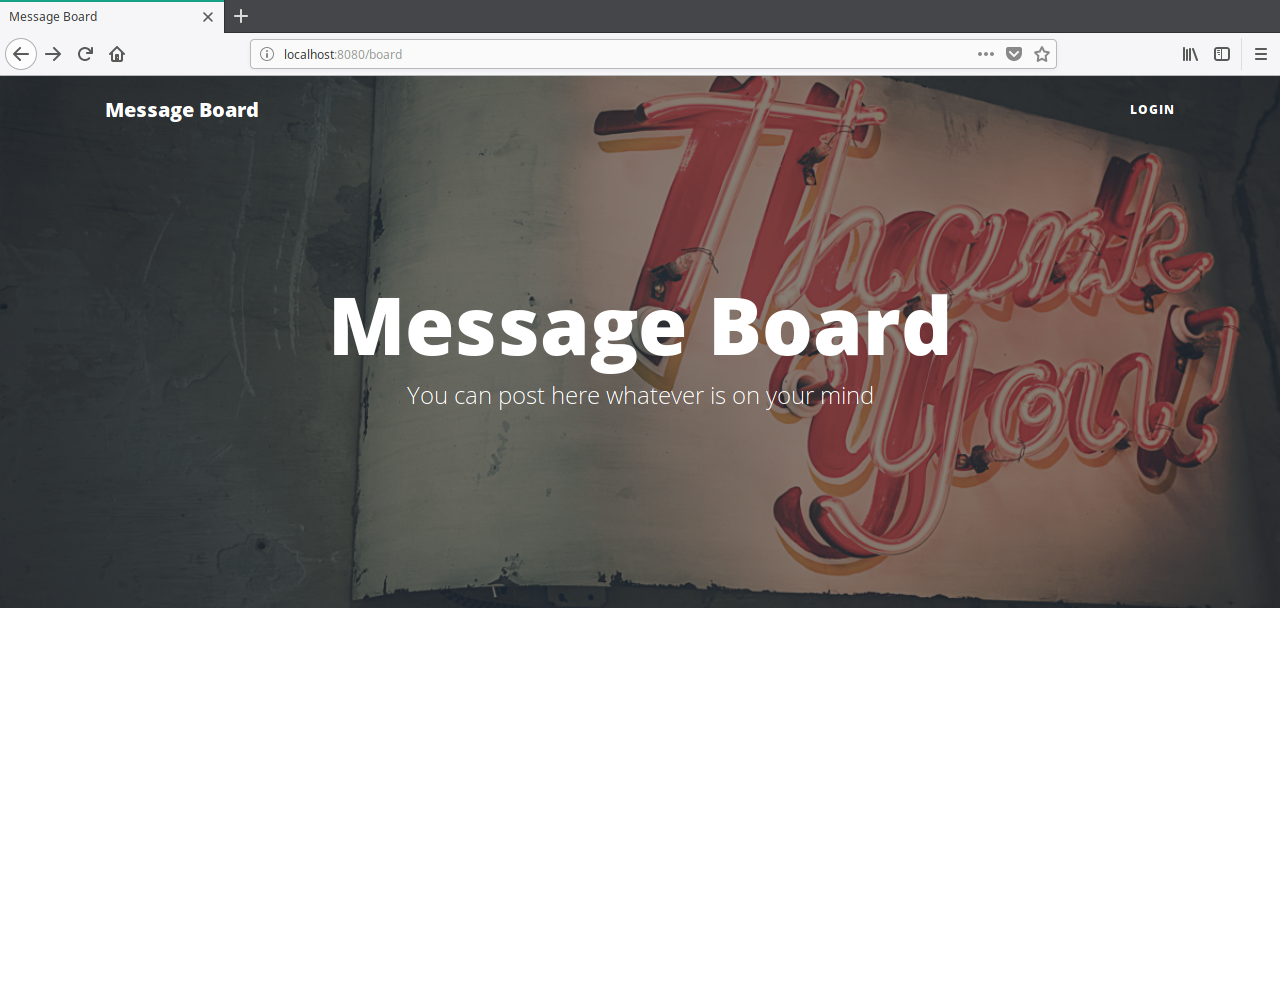
\includegraphics[scale=0.3]{board_guest.png}}
            \caption{Страница просмотра объявлений}
        \end{flushleft}
    \end{figure}
	\pagebreak
    \subsection{Вход в систему}
    После нажатия на кнопку логин, мы вводим имя пользователя и пароль.
    \begin{figure}[H]
        \begin{flushleft}
            \centerline{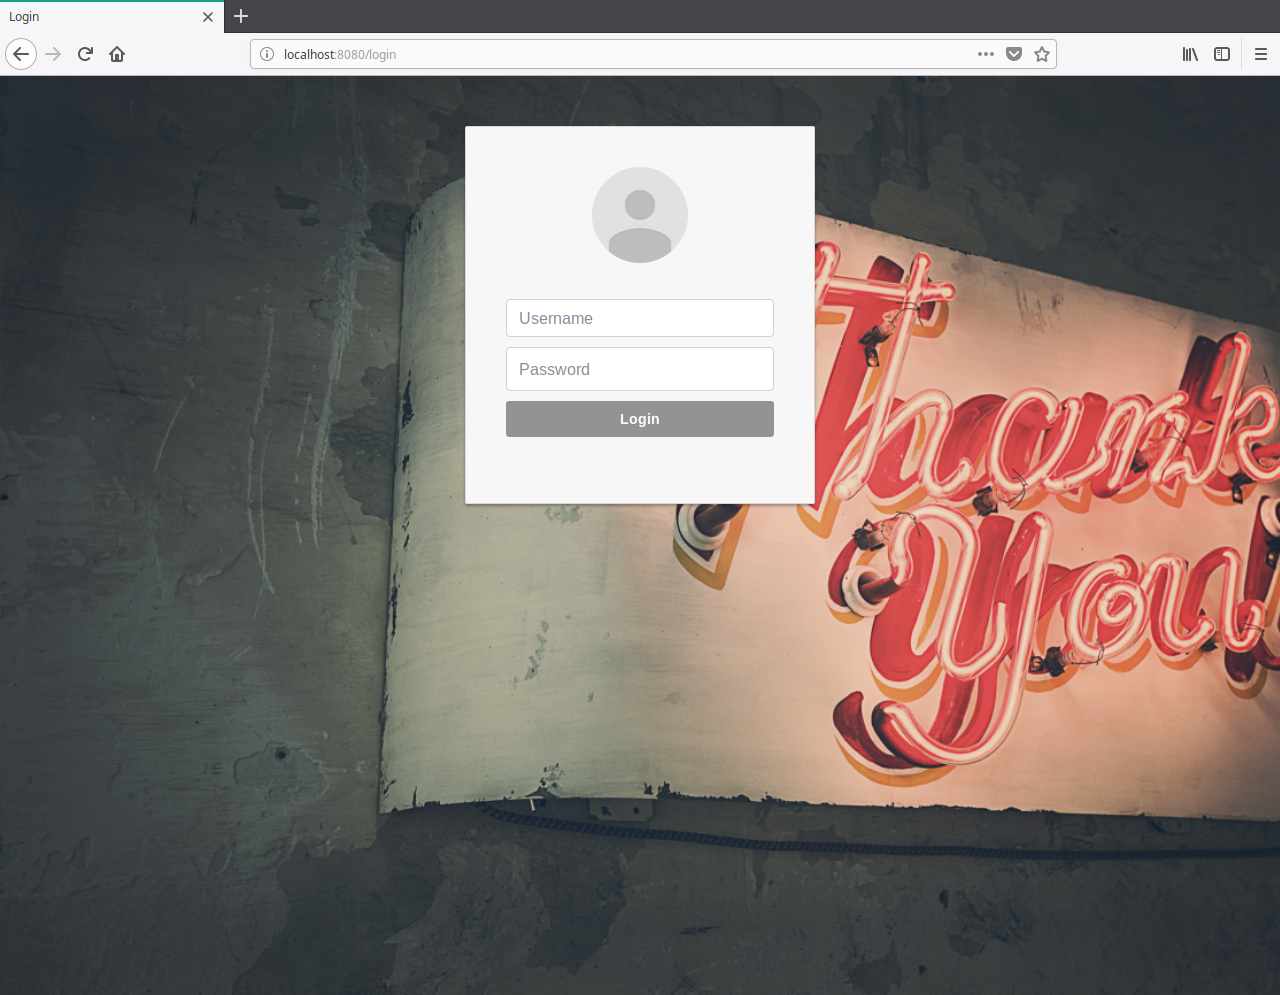
\includegraphics[scale=0.3]{login.png}}
            \caption{Ввод логина и пароля для входа в систему}
        \end{flushleft}
    \end{figure}
    При верно введенных логине и пароле, нас пересылает на доску объявлений уже как пользователя.
    \begin{figure}[H]
        \begin{flushleft}
            \centerline{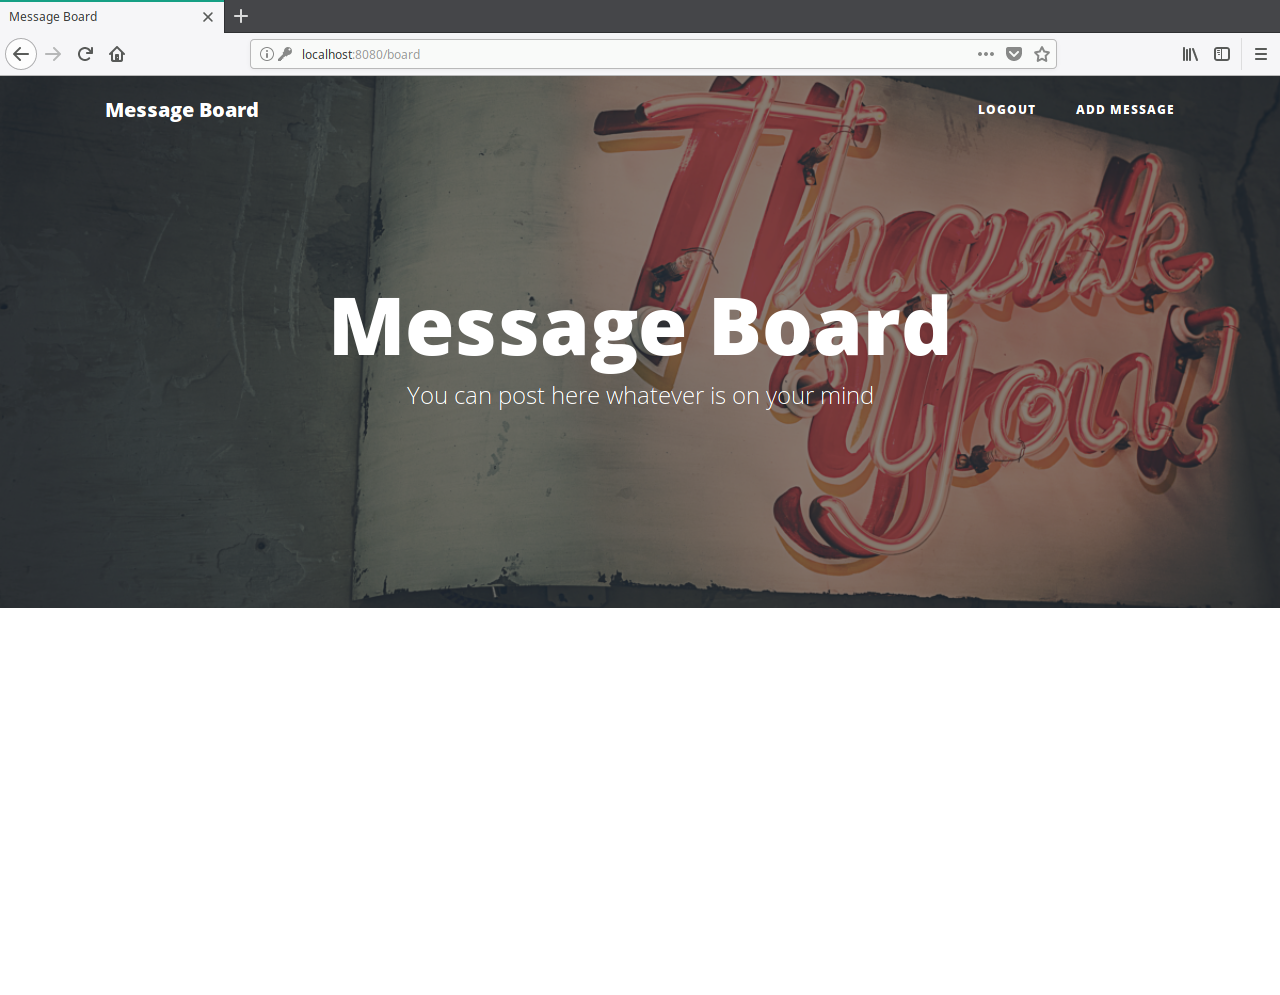
\includegraphics[scale=0.3]{afterlogin.png}}
            \caption{Вид доски объявлений после входа в систему}
        \end{flushleft}
    \end{figure}
   \pagebreak

    \subsection{Создание нового объявления}
	Если пользователь нажмёт кнопку создания нового объявления его перенаправят на страницу с формой нового объявления.
    \begin{figure}[H]
        \begin{flushleft}
            \centerline{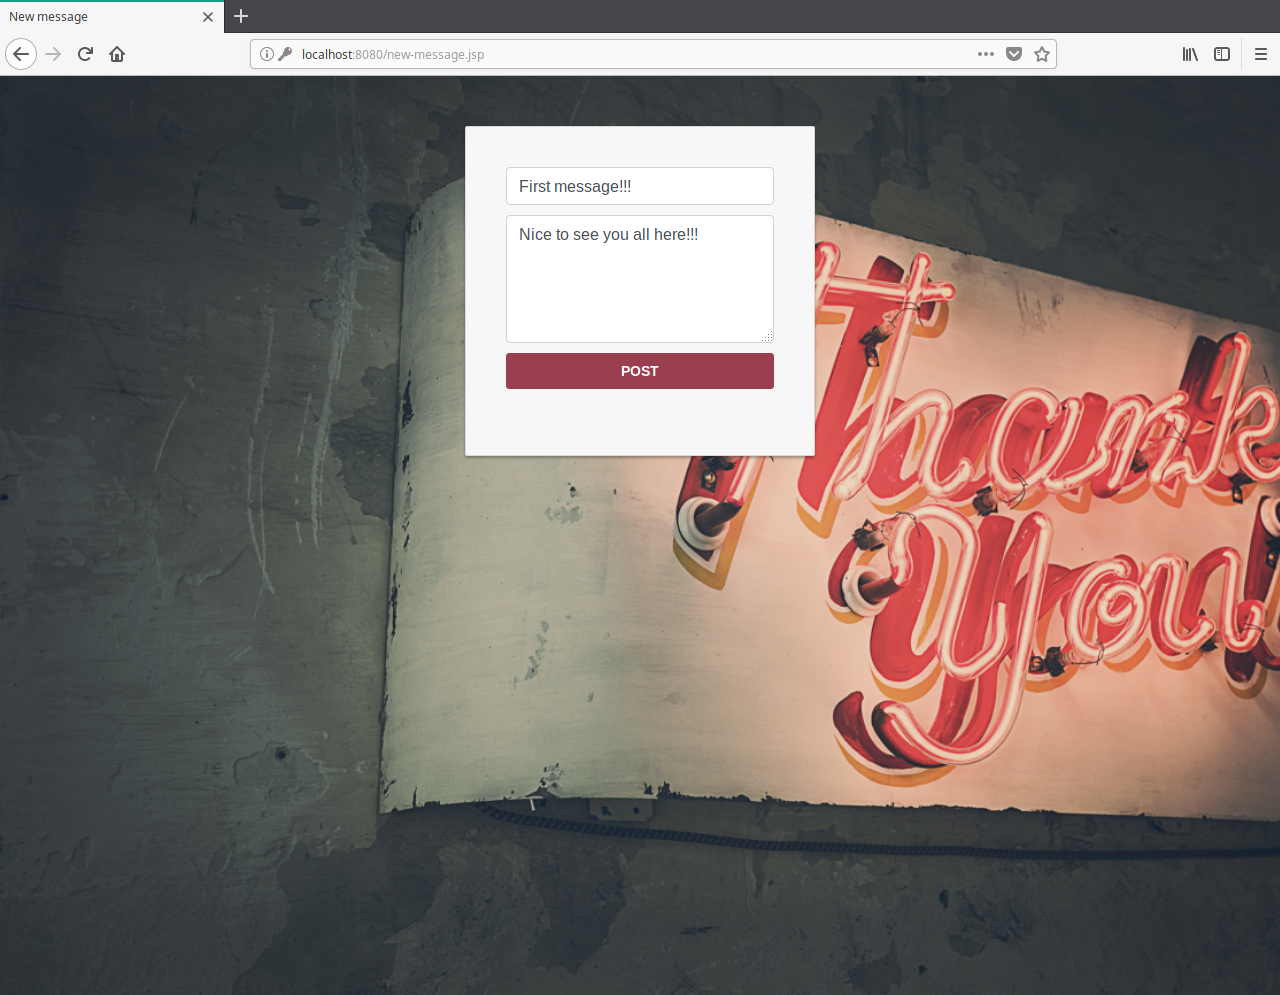
\includegraphics[scale=0.3]{newmessage.png}}
            \caption{Форма для создания объявления}
        \end{flushleft}
    \end{figure}

	После отправки нового объявления пользователя перенаправляет на страницу с объявлениями, где можно наблюдать новое объявление.
    \begin{figure}[H]
        \begin{flushleft}
            \centerline{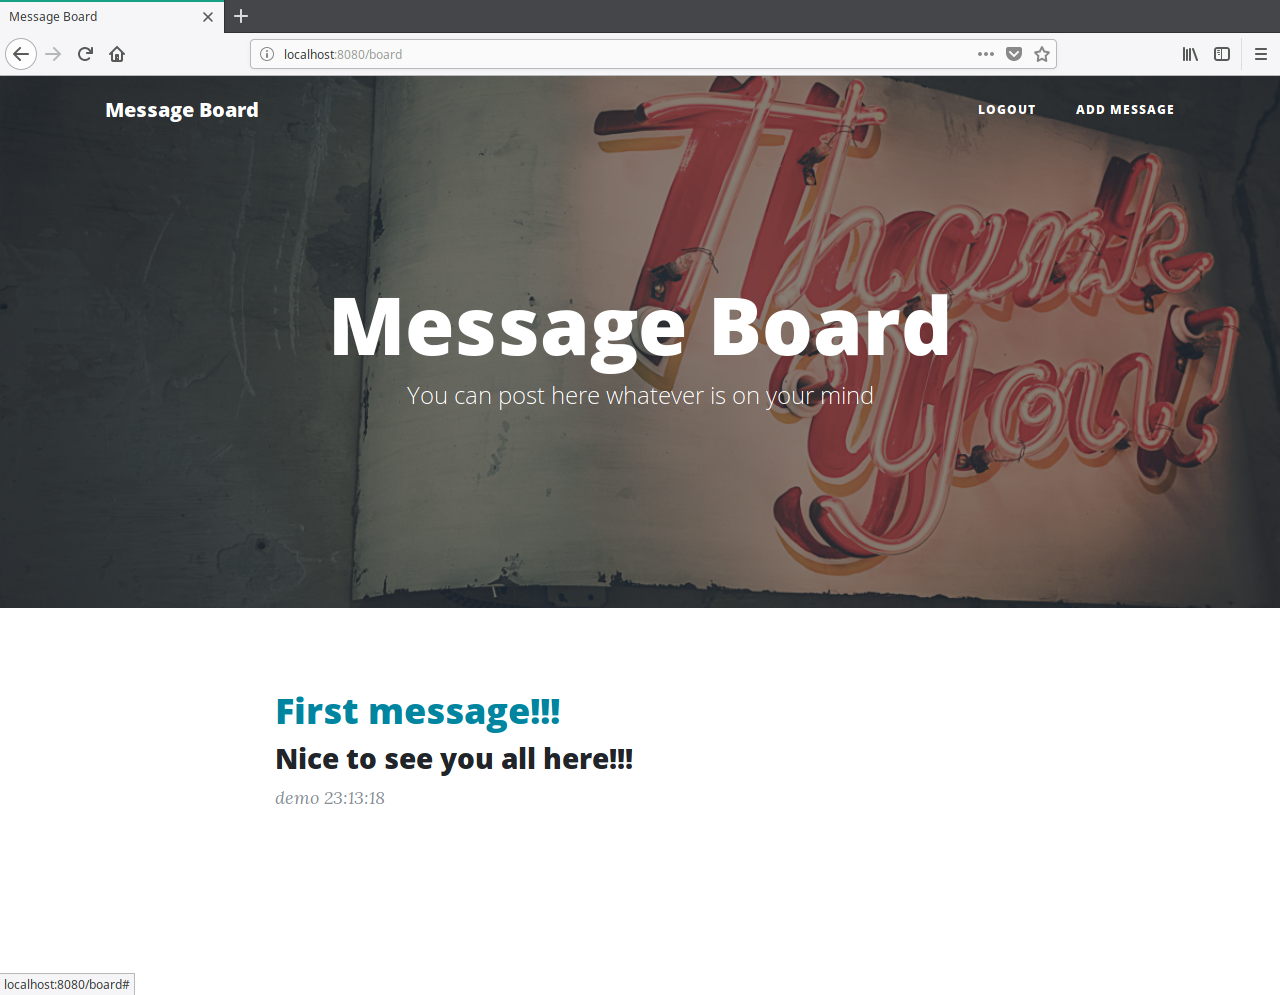
\includegraphics[scale=0.3]{user.png}}
            \caption{Новое объявление появилось в списке}
        \end{flushleft}
    \end{figure}

	\subsection{Страница администратора}
	Если при логине были введены логин и пароль суперпользователя и открыта страница с менеджментом пользователей появляется список всех пользователей.
    \begin{figure}[H]
        \begin{flushleft}
            \centerline{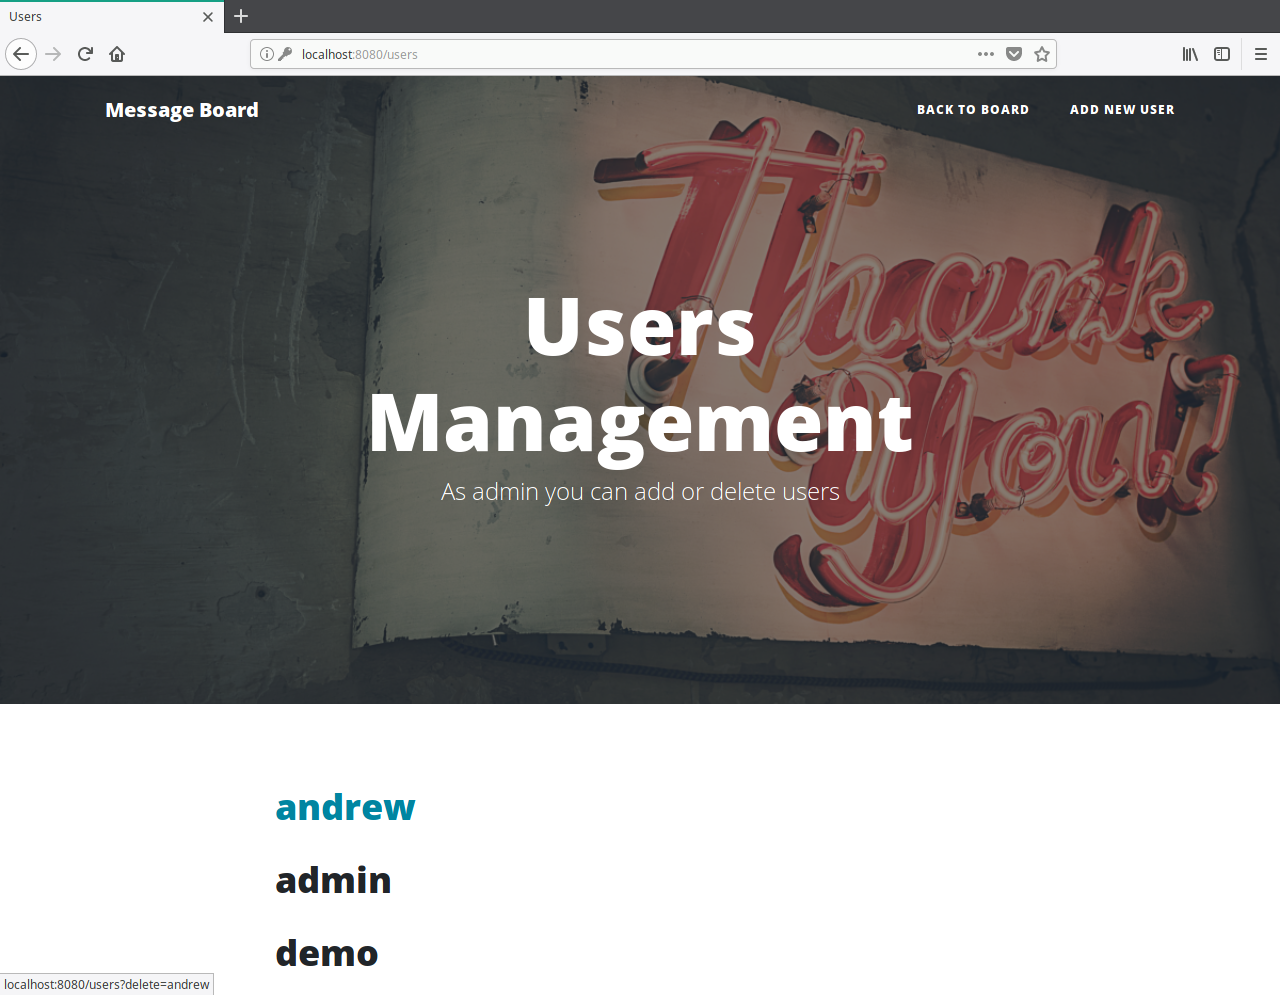
\includegraphics[scale=0.3]{admin.png}}
            \caption{Список всех пользователей}
        \end{flushleft}
    \end{figure}
    
    Кликнув по имени пользователя мы можем удалить его из списка пользователей, теперь ему нельзя войти в систему по прежнему логину.
    \begin{figure}[H]
        \begin{flushleft}
            \centerline{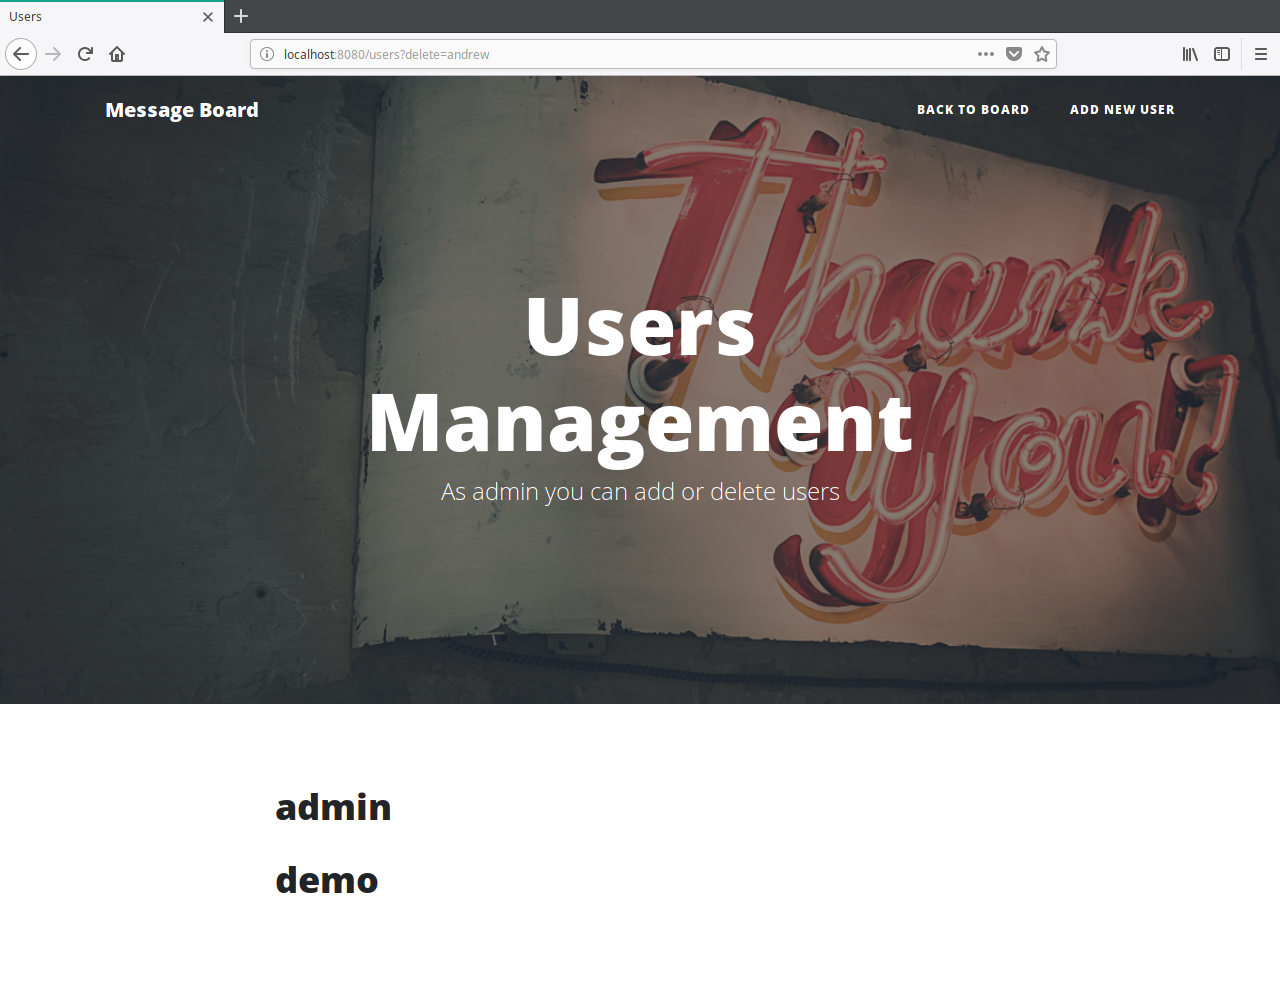
\includegraphics[scale=0.3]{deleteuser.png}}
            \caption{Список всех пользователей}
        \end{flushleft}
    \end{figure}


\end{document}